% ReadPast -- IEEE TCSVT submission (skeleton, 2026-11-04)
% Build: latexmk -pdf main.tex  (needs TeX Live with IEEEtran; or upload paper/ to Overleaf)
% Page budget (TCSVT: <=14 pages at submission incl. figures; overlength charges from page 12 -> aim for 11):
%   Abstract+Intro 1.5 | Related Work 1.5 | Method 2 | Experiments 4.5 | Limitations+Conclusion 0.5 | Refs ~1
\documentclass[journal]{IEEEtran}
\usepackage{amsmath,amssymb}
\usepackage{graphicx}
\usepackage{booktabs}
\usepackage{multirow}
\usepackage{xcolor}
\usepackage[hidelinks]{hyperref}
\usepackage{cite}
\graphicspath{{figs/}}

\newcommand{\todo}[1]{\textcolor{red}{[TODO: #1]}}
\newcommand{\method}{ReadPast}

\begin{document}

\title{\method{}: See the Present, Read the Past for Training-Free Streaming Video Question Answering}
% TODO: final title

\author{Ren~\todo{full name},~and~\todo{co-authors}%
\thanks{\todo{Affiliation, e-mail (TCSVT asks for affiliation and e-mail footnote).}}}

\markboth{IEEE Transactions on Circuits and Systems for Video Technology}%
{\method{}: Training-Free Streaming Video Question Answering}

\maketitle

% TCSVT: abstract 150--200 words. Draft below is ~180 words; numbers = round 17 (standard OVO = (BT+RT)/2).
\begin{abstract}
Streaming video question answering requires a model to answer about what is happening now and about what happened earlier, while the video keeps arriving.
A strong recent baseline, SimpleStream, feeds only the latest few frames to an off-the-shelf video large language model and already rivals memory-based systems on real-time questions, but it cannot answer questions whose evidence has left the window.
We present \method{}, a training-free, plug-in extension that keeps the visual input at the recent window and carries the past as text.
The same frozen model periodically writes a short caption of the stream into a timestamped timeline; a present/past gate reads only the question and decides whether the timeline is needed, with its threshold set without any labels by content-free calibration; and an abstention instruction is added only when the answer options contain an abstention choice.
On OVO-Bench, \method{} improves SimpleStream by 6.0, 5.7, 5.2, and 2.5 points on Qwen2.5-VL-7B, Qwen3-VL-8B, Qwen3-VL-4B, and LLaVA-OneVision-7B, without lowering real-time accuracy, and \todo{StreamingBench real-time and comparison with D-HSM under the same protocol, after round 18}.
\todo{One sentence on cost from the efficiency table (round 19).}
\end{abstract}

\begin{IEEEkeywords}
Streaming video understanding, video large language models, video question answering, training-free, memory, calibration.
\end{IEEEkeywords}
% TODO: choose EDICS category on ScholarOne (TCSVT requires at least one).

\section{Introduction}
\label{sec:intro}
% ~1.5 pages incl. Fig. 1 (fig1_teaser). Paragraph plan:

% P1 Task. Streaming video QA: questions arrive at arbitrary times; some ask about the present (real-time), some about
%    the past (backward). Benchmarks: OVO-Bench, StreamingBench. Cost/latency matter because the stream does not stop.
\todo{P1: streaming VQA setting and why it differs from offline long-video QA.}

% P2 Observation that motivates us. SimpleStream: recent 4 frames to a frozen VLM is a strong baseline, often better
%    than memory systems on real-time questions; but backward questions fail when evidence left the window.
%    Adding history *frames* hurts present perception (Qwen3-VL-8B: 4 history frames RT -4.03, 16 low-res frames -5.86;
%    text timeline -0.81; EXPERIMENTS.md "实验 B 结果"). -> keep frames for the present, use text for the past.
\todo{P2: SimpleStream is strong; history frames dilute present perception; text does not.}

% P3 Two questions this raises: (i) when to read the past without labels or task names; (ii) how to make the model
%    say "cannot answer" without hurting answerable questions (uniform abstention instruction hurts 3/4 backbones).
\todo{P3: the two design questions (when to read; when to allow abstention).}

% P4 Method in one paragraph (Fig. 1 teaser): self-written timeline + calibrated present/past gate + conditional
%    abstention instruction (instruction text from D-HSM \cite{dhsm}; our change is when it is applied).
\todo{P4: ReadPast overview.}

% P5 Results headline: +6.03/+5.68/+5.18/+2.45 OVO over SimpleStream on 4 backbones, RT not lowered;
%    same-protocol comparison with D-HSM (round 18); cost (round 19).
\todo{P5: headline results.}

% Contributions (TCSVT style: 3--4 bullets, each verifiable by a table/figure):
\begin{itemize}
  \item A training-free, plug-in extension of recent-frame streaming baselines that keeps the visual input at the
        recent window and carries the past as a self-written text timeline; we show that text history preserves
        real-time accuracy whereas history frames lower it (Sec.~\ref{sec:exp-analysis}).
  \item A question-only present/past gate whose threshold is set without labels by content-free calibration
        \cite{zhao2021calibrate}, performing on par with gates calibrated on labeled synthetic queries
        \todo{wording after final gate comparison table} (Sec.~\ref{sec:method-gate}).
  \item An analysis showing that an abstention instruction should be conditioned on the answer options:
        applying it only when an abstention option exists outperforms applying it to every question on three of four
        backbones (Sec.~\ref{sec:exp-ablation}).
  \item Experiments on four backbones and two benchmarks, with same-protocol reruns of public training-free methods
        (Sec.~\ref{sec:exp-main}).
\end{itemize}

\section{Related Work}
\label{sec:related}
% ~1.5 pages. Reading list: reports/TCSVT 论文写作 必读文献.md (in progress). Existing survey: RELATED.md.
% Rule: methods in comparison tables must have public code; others are cited only.

\subsection{Streaming Video Large Language Models}
% Online/streaming VideoLLMs (KV-cache, memory banks, retrieval) and their benchmarks (OVO-Bench, StreamingBench).
% SimpleStream \cite{simplestream} as the recent-window baseline; trained methods (SelectStream, SPARE, ...) cited.
\todo{streaming VideoLLMs; benchmarks; trained vs training-free.}

\subsection{Memory for Long and Streaming Video}
% Visual-token memory vs text memory. Caption/text memory for long video (LLoVi, VideoAgent, ...);
% streaming text memory: D-HSM \cite{dhsm} (hub-and-spoke entity memory), FOLIO, StreamScout, DeltaStreamer.
% Our position: a plain timeline written by the same frozen model; contribution is not the memory structure.
\todo{text vs visual memory; where ReadPast sits.}

\subsection{Deciding When to Read the Past}
% Adaptive retrieval in RAG (Self-RAG, Adaptive-RAG, FLARE, SKR, ...); streaming gates: ShallowStream
% \cite{shallowstream} (query-logit gate, threshold on 200 synthetic labeled queries), FlashBack, WRWS, StreamScout.
% Ours: question-only, threshold label-free via content-free inputs.
\todo{when-to-retrieve gates and how their thresholds are set.}

\subsection{Calibration and Abstention}
% Contextual calibration \cite{zhao2021calibrate}, PMI/domain-context/batch calibration; we calibrate a binary routing
% threshold rather than answer priors. Abstention/unanswerable QA; D-HSM's instruction; our conditional use.
\todo{calibration lineage; abstention lineage.}

\section{Method}
\label{sec:method}
% ~2 pages incl. Fig. 2 (fig2_method, double column).

\begin{figure*}[t]
  \centering
  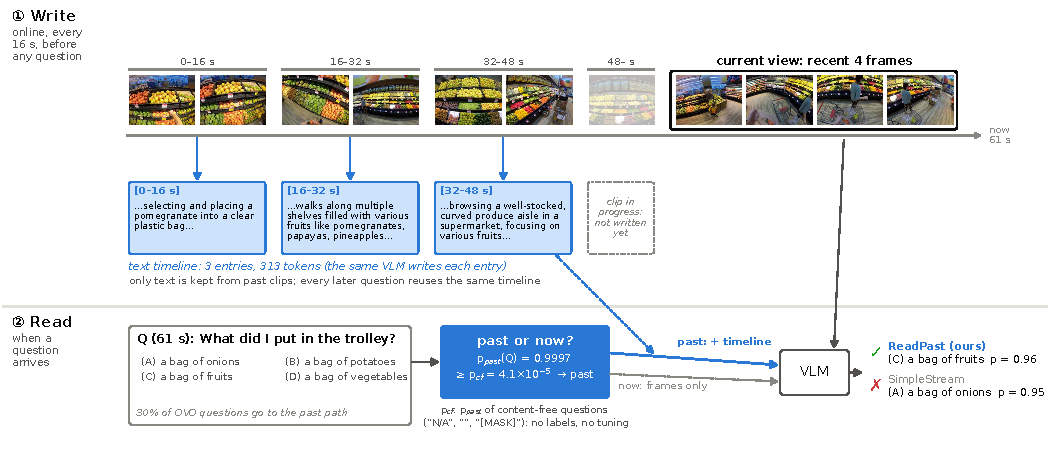
\includegraphics[width=\textwidth]{fig2_method.pdf}
  \caption{Overview of \method{}. \todo{caption}}
  \label{fig:method}
\end{figure*}

\subsection{Problem Setup and the Recent-Window Baseline}
\label{sec:method-setup}
% Stream V, question q at time t with options O. SimpleStream: answer from the last N=4 frames (1 fps sampling).
% Notation for the answer model f, recent frames F_t.
\todo{notation; SimpleStream as $f(F_t, q, O)$.}

\subsection{Self-Written Timeline}
\label{sec:method-timeline}
% Every s=16 s, the same frozen VLM captions 8 frames sampled uniformly in the segment -> (t0, t1, text).
% Timeline M_t = all captions with t1 <= t, prepended before the recent frames (placement ablation: round 10, "before"
% better on 3 backbones). Cost: one 8-frame generation per 16 s of stream; mean 1264 timeline tokens on OVO.
% Writer prompt in appendix.
\todo{writer, schedule, prompt, placement.}

\subsection{Present/Past Gate with Content-Free Calibration}
\label{sec:method-gate}
% Fixed routing prompt on the question text only (no frames, no options: an "Unable to answer" option would leak the task) -> p_past = P("past") / (P("past")+P("now")).
% Threshold p_cf = mean p_past over content-free questions {"N/A", "", "[MASK]"}; read timeline iff p_past >= p_cf.
% One extra forward pass of the text-only prompt per question. Fig. 3 (fig3_calibration): log-odds distributions,
% fixed 0.5 vs p_cf, read rates. Be honest: on LLaVA-OV p_cf is low (RT read rate 40%).
\todo{gate definition, calibration, Fig.~3.}

\subsection{Conditional Abstention Instruction}
\label{sec:method-abstain}
% Instruction text from D-HSM \cite{dhsm}: choose a content option only when evidence supports it, otherwise the
% abstention option. Applied iff O contains an abstention option (e.g., "Unable to answer"); otherwise prompt unchanged.
% Rationale: on questions without such an option the instruction only adds a prior toward refusing / changes answers.
\todo{instruction, trigger rule, rationale.}

\subsection{Cost}
\label{sec:method-cost}
% Write cost amortized per stream second; per-question extra cost = gate forward + timeline prefill. Numbers in
% Sec.~\ref{sec:exp-efficiency}.
\todo{complexity summary.}

\section{Experiments}
\label{sec:exp}
% ~4.5 pages. Report point gains, no significance tests. Standard OVO avg + per-task only (no extra HLD analysis).

\subsection{Setup}
\label{sec:exp-setup}
% Benchmarks: OVO-Bench backward (EPM, ASI, HLD) + real-time (OCR, ACR, ATR, STU, FPD, OJR), 1468 MCQ (631 BT + 837 RT);
%   avg = (BT + RT)/2, Forward not used. StreamingBench real-time, 2500 questions / 500 videos.
% Backbones: Qwen2.5-VL-7B, Qwen3-VL-8B (development), Qwen3-VL-4B (held-out), LLaVA-OneVision-7B (report only).
% Implementation: 1 fps, recent 4 frames, 16 s / 8-frame captions, greedy decoding, scorer = generated letter.
% Baselines: SimpleStream (our rerun, 64.75 vs paper 65.13 on Qwen2.5); D-HSM (public code, same protocol, round 18);
%   ShallowStream (paper values, its own protocol -- marked).
\todo{setup text.}

\subsection{Main Results}
\label{sec:exp-main}
\begin{table*}[t]
  \centering
  \caption{OVO-Bench results (standard avg $=(\mathrm{BT}+\mathrm{RT})/2$). Point gains over SimpleStream in parentheses.
  \todo{per-task RT columns from \texttt{kfs/analyze\_round17.py}; D-HSM rows after round 18.}}
  \label{tab:main-ovo}
  \begin{tabular}{llccccc}
    \toprule
    Backbone & Method & EPM & ASI & HLD & RT & Avg \\
    \midrule
    \multirow{2}{*}{Qwen2.5-VL-7B} & SimpleStream & 53.5 & 61.5 & 40.3 & 77.7 & 64.75 \\
                                   & \method{}    & 53.9 & 64.2 & 73.1 & 77.8 & 70.78 (+6.03) \\
    \midrule
    \multirow{2}{*}{Qwen3-VL-8B}   & SimpleStream & 52.2 & 58.1 & 51.6 & 81.4 & 67.66 \\
                                   & \method{}    & 51.9 & 69.6 & 73.7 & 81.7 & 73.34 (+5.68) \\
    \midrule
    \multirow{2}{*}{Qwen3-VL-4B}   & SimpleStream & 54.6 & 57.4 & 51.6 & 80.3 & 67.42 \\
                                   & \method{}    & 54.2 & 62.8 & 78.0 & 80.2 & 72.60 (+5.18) \\
    \midrule
    \multirow{2}{*}{LLaVA-OV-7B}   & SimpleStream & 55.6 & 54.7 & 20.4 & 74.7 & 59.15 \\
                                   & \method{}    & 58.3 & 57.4 & 31.7 & 74.1 & 61.60 (+2.45) \\
    \bottomrule
  \end{tabular}
\end{table*}
% StreamingBench real-time (no abstention options -> instruction never triggers): ReadPast - SimpleStream =
%   -0.20 / +1.36 / +1.48 / +0.28 (Qwen2.5: 79.76 -> 79.56; Qwen3-8B: 80.28 -> 81.64; LLaVA: 74.64 -> 74.92; 4B: TODO).
\todo{SB table or SB columns; text.}

\subsection{Comparison with Training-Free Methods}
\label{sec:exp-compare}
% D-HSM same protocol (round 18, kfs/analyze_round18_dhsm.py) + D-HSM paper values; ShallowStream paper values
% (Qwen3-8B OVO 69.5 / SB-RT 78.2; LLaVA-OV 62.2 / 75.5), marked "paper value, own protocol".
\todo{after round 18.}

\subsection{Ablation Study}
\label{sec:exp-ablation}
% Table: 2x2 (timeline+gate on/off x conditional instruction on/off) + "instruction on every question" row
% (round 18: Delta cond - always = -0.52 / +1.75 / +1.24 / +0.30). Gate variants (fixed 0.5 vs p_cf; read-all;
% ShallowStream gate). Timeline placement (before vs after recent frames, round 10).
\todo{ablation tables.}

\subsection{Analysis}
\label{sec:exp-analysis}
% (1) Text vs history frames (Qwen3-8B: RT -0.81 vs -4.03 / -5.86; Qwen2.5 similar).
% (2) Timeline content vs foreign timeline (content control): EPM +6.7 / +5.4 own minus foreign.
% (3) Memory reach: gains concentrated within ~90 s of the evidence -> limitation.
% (4) Gate calibration (Fig. 3).
\begin{figure*}[t]
  \centering
  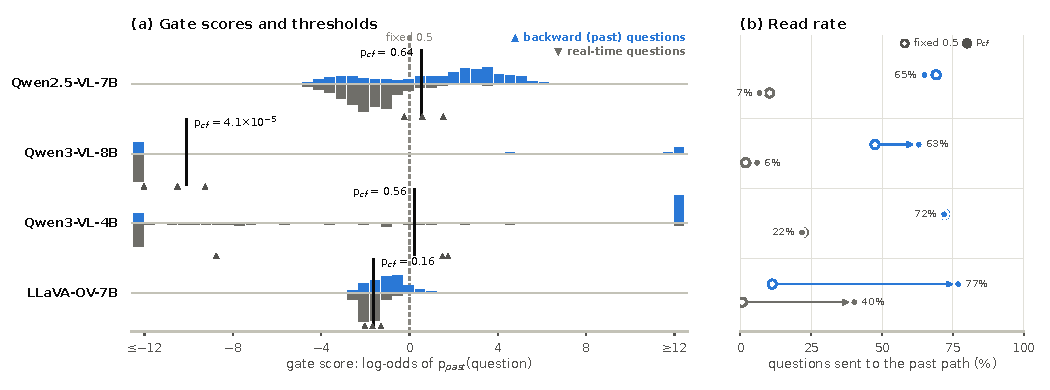
\includegraphics[width=\textwidth]{fig3_calibration.pdf}
  \caption{Content-free calibration of the present/past gate on four backbones. \todo{caption}}
  \label{fig:calib}
\end{figure*}
\todo{analysis text.}

\subsection{Efficiency}
\label{sec:exp-efficiency}
% Round 19 (plan in EXPERIMENTS.md): write cost per stream second (real-time factor), per-question latency
% (gate + answer), peak GPU memory, timeline tokens; SimpleStream / ReadPast / D-HSM on the same GPU, exclusive.
\todo{efficiency table.}

\subsection{Qualitative Results and Failure Cases}
\label{sec:exp-qual}
\todo{2--3 examples: a backward question answered from the timeline; a real-time question kept on frames; a failure
(evidence older than the reach / not written).}

\section{Limitations}
\label{sec:limits}
% Memory reach is short (gains concentrated within ~1.5 min of the evidence); write coverage is the bottleneck
% (information never written cannot be read); calibration transfers less well to LLaVA-OV (RT read rate 40%);
% the abstention instruction is borrowed from D-HSM, our change is only when it is applied.
\todo{limitations.}

\section{Conclusion}
\label{sec:conclusion}
\todo{conclusion.}


\bibliographystyle{IEEEtran}
\bibliography{refs}

\end{document}
